\chapter{Electrostatics} \label{chap:Electrostatics}
		\section{Electrostatic Charge} \index{Electrostatic Charge} \index{Charge}
		
		You've probably experienced electrostatic charges - sometimes we just call it static - in everyday life.  Dragging your shoes on carpet, rubbing  balloon on your hair, and even just putting on a piece of clothing can cause electrostatic charges to build up, causing articles to cling together, your hair to get frizzy, and can even cause small sparks. 
		
		Most electrical charges we encounter in everyday life are due to imbalances of protons and electrons. Electrons are capable of moving from atom to atom under the right conditions.  However, protons are stuck in the nucleus of an atom and do not move unless nuclear reactions are taking place.  Thus, most electrical charges we encounter in actual life are due to electrons being transferred from one object to another.   
		
		The units for charge are Coulombs (C), and it is represented by the variable q.  You may remember from chemistry that protons have small positive charges and electrons have small negative charges.  Table \ref{table:elementarycharges} shows the charge of each of the elementary particles that make up normal matter:
		
		\index{Elementary Charge} \index{Charge, Elementary}
		\begin{center}
			\begin{table}[!h]
				\centering
			\caption{Elementary Charges} \label{table:elementarycharges} 
				\begin{tabular}{|c|c|c|}
					\hline
					\textbf{Particle} & \textbf{Charge}	& \textbf{Mass} \\
					\hline
					Proton & $1.602\times 10^{-19}$ C  & $1.673\times10^{-27}$ kg\\
					\hline
					Electron & $-1.602\times 10^{-19}$ C  & $9.109 \times 10^{-31} $ kg  \\
					\hline
					Neutron & $0$ C  & $1.675 \times 10^{-31} $ kg  \\
					\hline
				\end{tabular}
				
			\end{table}
		\end{center}		
		
	You may notice that the charge of an electron and a proton are exactly the same with the only difference being a negative sign for the electron.  Thus a Hydrogen atom, made of 1 proton and 1 electron will have a total charge of zero coulombs.  In fact, any combination of the same number of protons and electrons will have no charge. 
	
	You should also note that 1 coulomb of electrostatic charge is a large amount.  Most charges we encounter in everyday life might be 1 millionth or even 1 billionth of a coulomb. 
	
	

	\section{Coulomb's Law and Electrostatic Force} \index{Coulomb's Law} \index{Electrostatic Force}

When two charged objects interact, it generates a force.  This force, often called electrostatic force, is repulsive for charges with the same sign, whereas it is attractive for two charges with opposite signs.  So two positive charges will repel, as will two negative charges, but a positive charge will be attracted to a negative charge.  


To determine the about of force that will be exerted one charged particle due to another charged particle, we use \textbf{Coulomb's Law}:
\begin{mdframed}[backgroundcolor=orange!20!white]

	\begin{equation}
	F = \frac{kq_1q_2}{r^2}
	\label{equation:coulombslaw}
	\end{equation}
\end{mdframed}	
	In this equation, $q_1$ and $q_2$ are the charges of the particles, r is the distance between the charges, and k is \textbf{Coulomb's Constant}.  Coulomb's Constant is a universal constant, meaning its value does not change.  The value of coulomb's constant is $k \approx \SI[per-mode = symbol]{9e9}{\N\m^2\per\coulomb^2}$.
	
	It is also important to note that this equation has a non-intuitive sign convention.  Repulsive forces will be postive, and attractive forces will be negative.  If forces calculated using Coulomb's Law need to be used in further calculations, be sure assign a positive or negative to the calculated force according to the direction the force is actually in.  
	
	\begin{mdframed}[backgroundcolor=blue!10!white]
		\begin{center}
			
			
			\textbf{Example \thesection.1}	
		\end{center}
		\vspace{0.1in}
		\textbf{Problem: } A positive charge of $\SI{3}{\micro\coulomb}$ and a negative charge of $\SI{-4}{\micro\coulomb}$ are separated by a distance of 0.3 meters.  What is the electrostatic force felt by the positive charge due to the negative charge?
		
		\vspace{0.2in}
		
		
		
		
		
		\textbf{Solution:} 
		Begin by drawing a diagram of the situation: 
		
		
			\begin{center}
			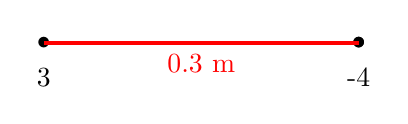
\begin{tikzpicture}
			\coordinate (A) at (0,0);
			\coordinate (B) at (4,0);
			\node[label=below:{\SI{3}{\micro \coulomb}}] at (A) {$\bullet$};
			\node[label=below:{\SI{-4}{\micro \coulomb}}] at (B) {$\bullet$};
			\node at (B) {$\bullet$};
			\draw  [red, ultra thick] (A) -- node[below] {0.3 m} (B) ; 
			
			\end{tikzpicture}   
			\end{center}			

		We also need to convert the charges into scientific notation:
		
		\begin{equation*}
		q_1 = \SI{3}{\micro\coulomb} = \SI{3e-6}{\coulomb}
		\end{equation*}	
		\begin{equation*}
		q_2 = \SI{-4}{\micro\coulomb} = \SI{-4e-6}{\coulomb}
		\end{equation*}	
		
		Note: It does not matter which charge is $q_1$ and which is $q_2$.  Either way will yield the same answer.  
		
		Now, we can use Coulomb's Law, equation \ref{equation:coulombslaw} to calculate the force:
		
			\begin{equation*}
		F = \frac{kq_1q_2}{r^2} = \frac{(\SI{9e9}{\N\m^2\per\coulomb^2})(\SI{3e-6}{\coulomb})(\SI{-4e-6}{\coulomb})}{(\SI{0.3}{\m})^2} = \boxed{\SI{-1.2}{\N}}
		\end{equation*}
		
		The negative on the answer does not indicate that the force it to the left.  Rather, it indicates that this is an attractive force.  Thus, the $\SI{3}{\micro\coulomb}$ charge feels a 1.2 N force directed to the \textit{right}, whereas the $\SI{-4}{\micro\coulomb}$ charge feels a 1.2 N force directed to the \textit{left}.
		
	\end{mdframed}
	
	
	
	
	
	
	\section{Electrostatic Potential Energy}
	\index{Electrostatic Potential Energy}
	\index{Potential Energy, Electrostatic}
	
	When two electrostatically charged objects are brought near each other, Coulomb's Law states that they will put a force on each other.  If the charged particles are then released, they will accelerate.  This means that two charged particles that are close enough to affect each other must have potential energy.  The formula to calculate electrostatic potential energy is:
	
	
	\begin{mdframed}[backgroundcolor=orange!20!white]
		
		\begin{equation}
		U_E = \frac{kq_1q_2}{r}
		\label{equation:electrostaticpotentialenergy}
		\end{equation}
	\end{mdframed}	
	
	
	
	
	\section{Electric Field} \index{Electric Field} \index{Electrostatic Field}
	
		\begin{mdframed}[backgroundcolor=orange!20!white]
		
		\begin{equation}
		{E} = \frac{kq}{r^2}
		\label{equation:electrostaticfield}
		\end{equation}
	\end{mdframed}	
	
	
	
	\section{Electric Potential and Voltage}
	
		\begin{mdframed}[backgroundcolor=orange!20!white]
	
	\begin{equation}
	V = \frac{kq}{r}
	\label{equation:electrostaticpotential}
	\end{equation}
\end{mdframed}	
	
	\section{Capacitors}
		\subsection{Construction of Capacitors}
		\subsection{Capacitors in Circuits}
		
	
	
	

	


